% TALK ABOUT HYDRA AND HOW THE ORGANISMS CAN REGENERATE PARTS OF ITS BODY.

\section{Hydra Morphogenesis and regenerative properties}

Hydras are fascinating organisms. Despite their rather small size (roughly 5mm in average), they are capable of extraordinary regenerative properties that allows them to fully reconstruct their body out of a very small portion of tissue (see figure \ref{hydraregen}) 

\begin{figure}
\label{hydraregen}
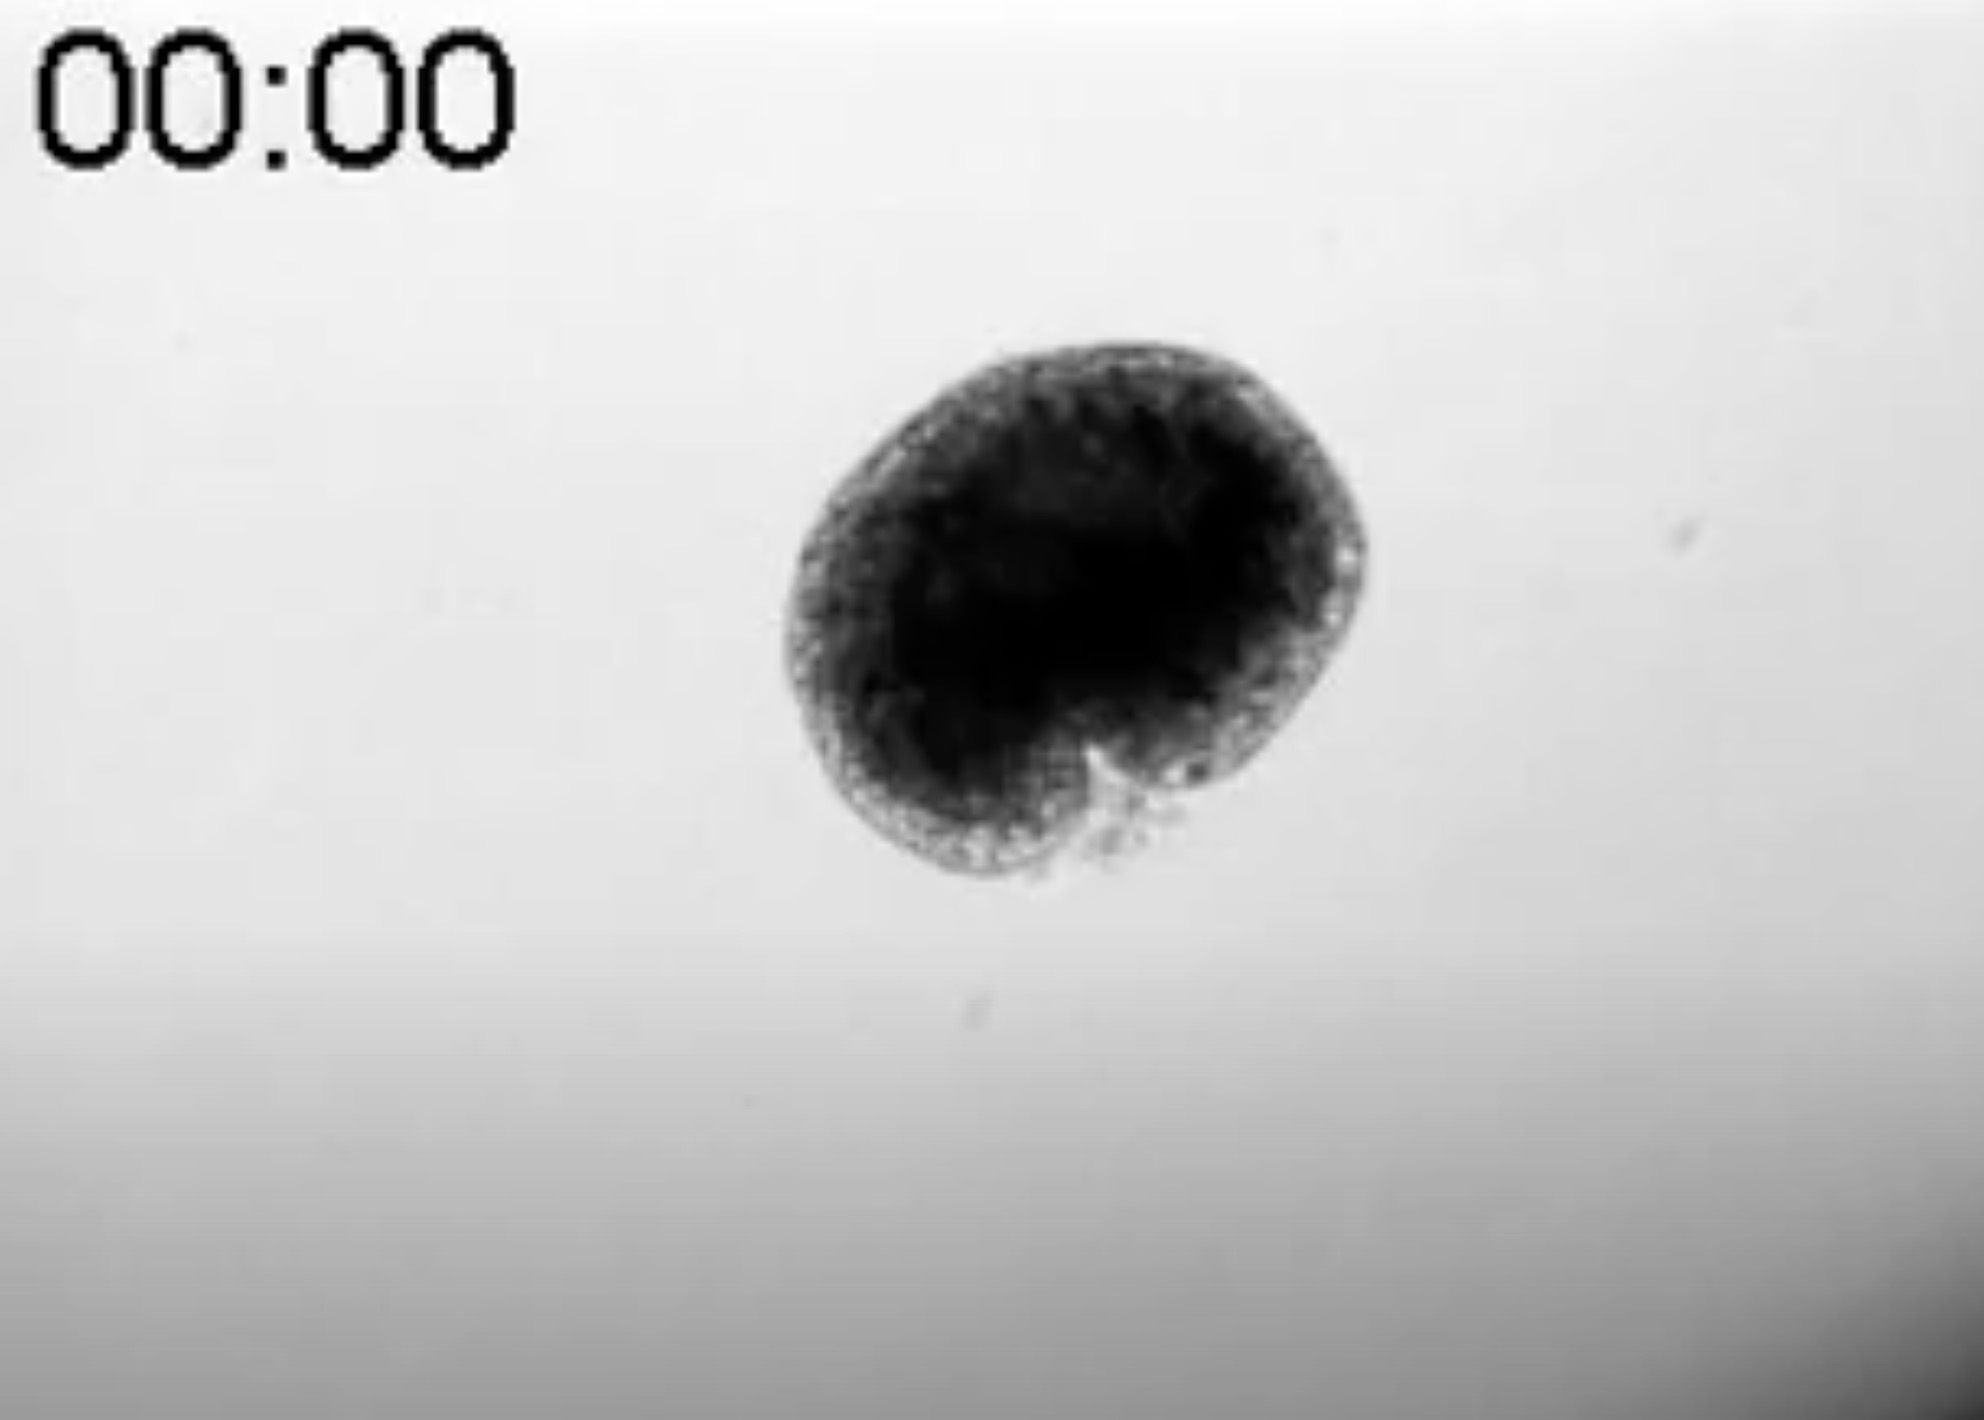
\includegraphics[width=0.19\textwidth]{figures/hydra_growth1}
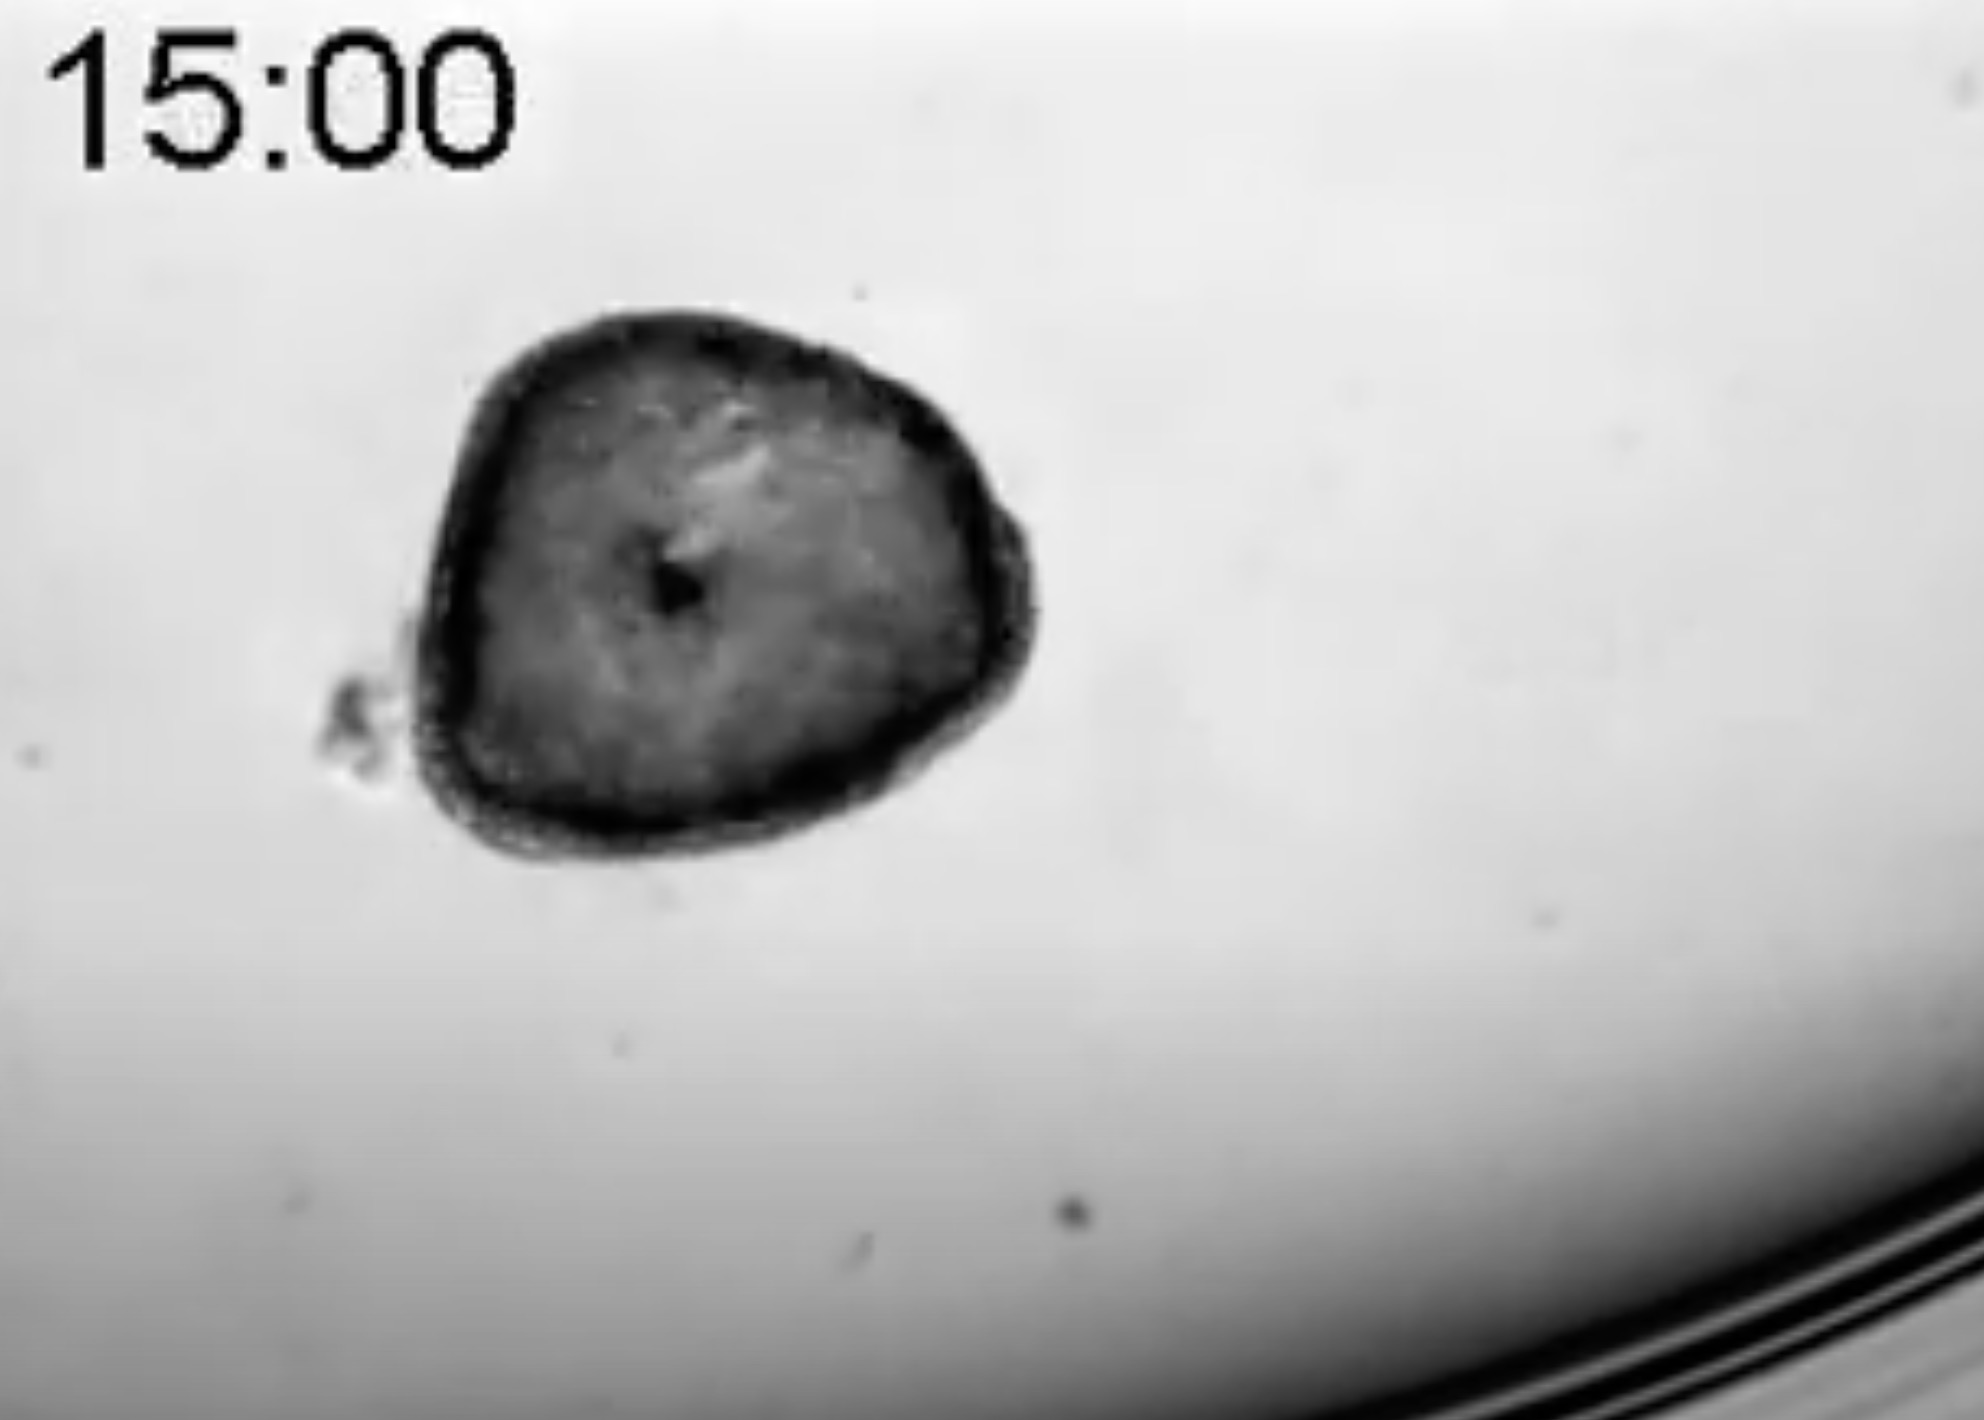
\includegraphics[width=0.19\textwidth]{figures/hydra_growth2}
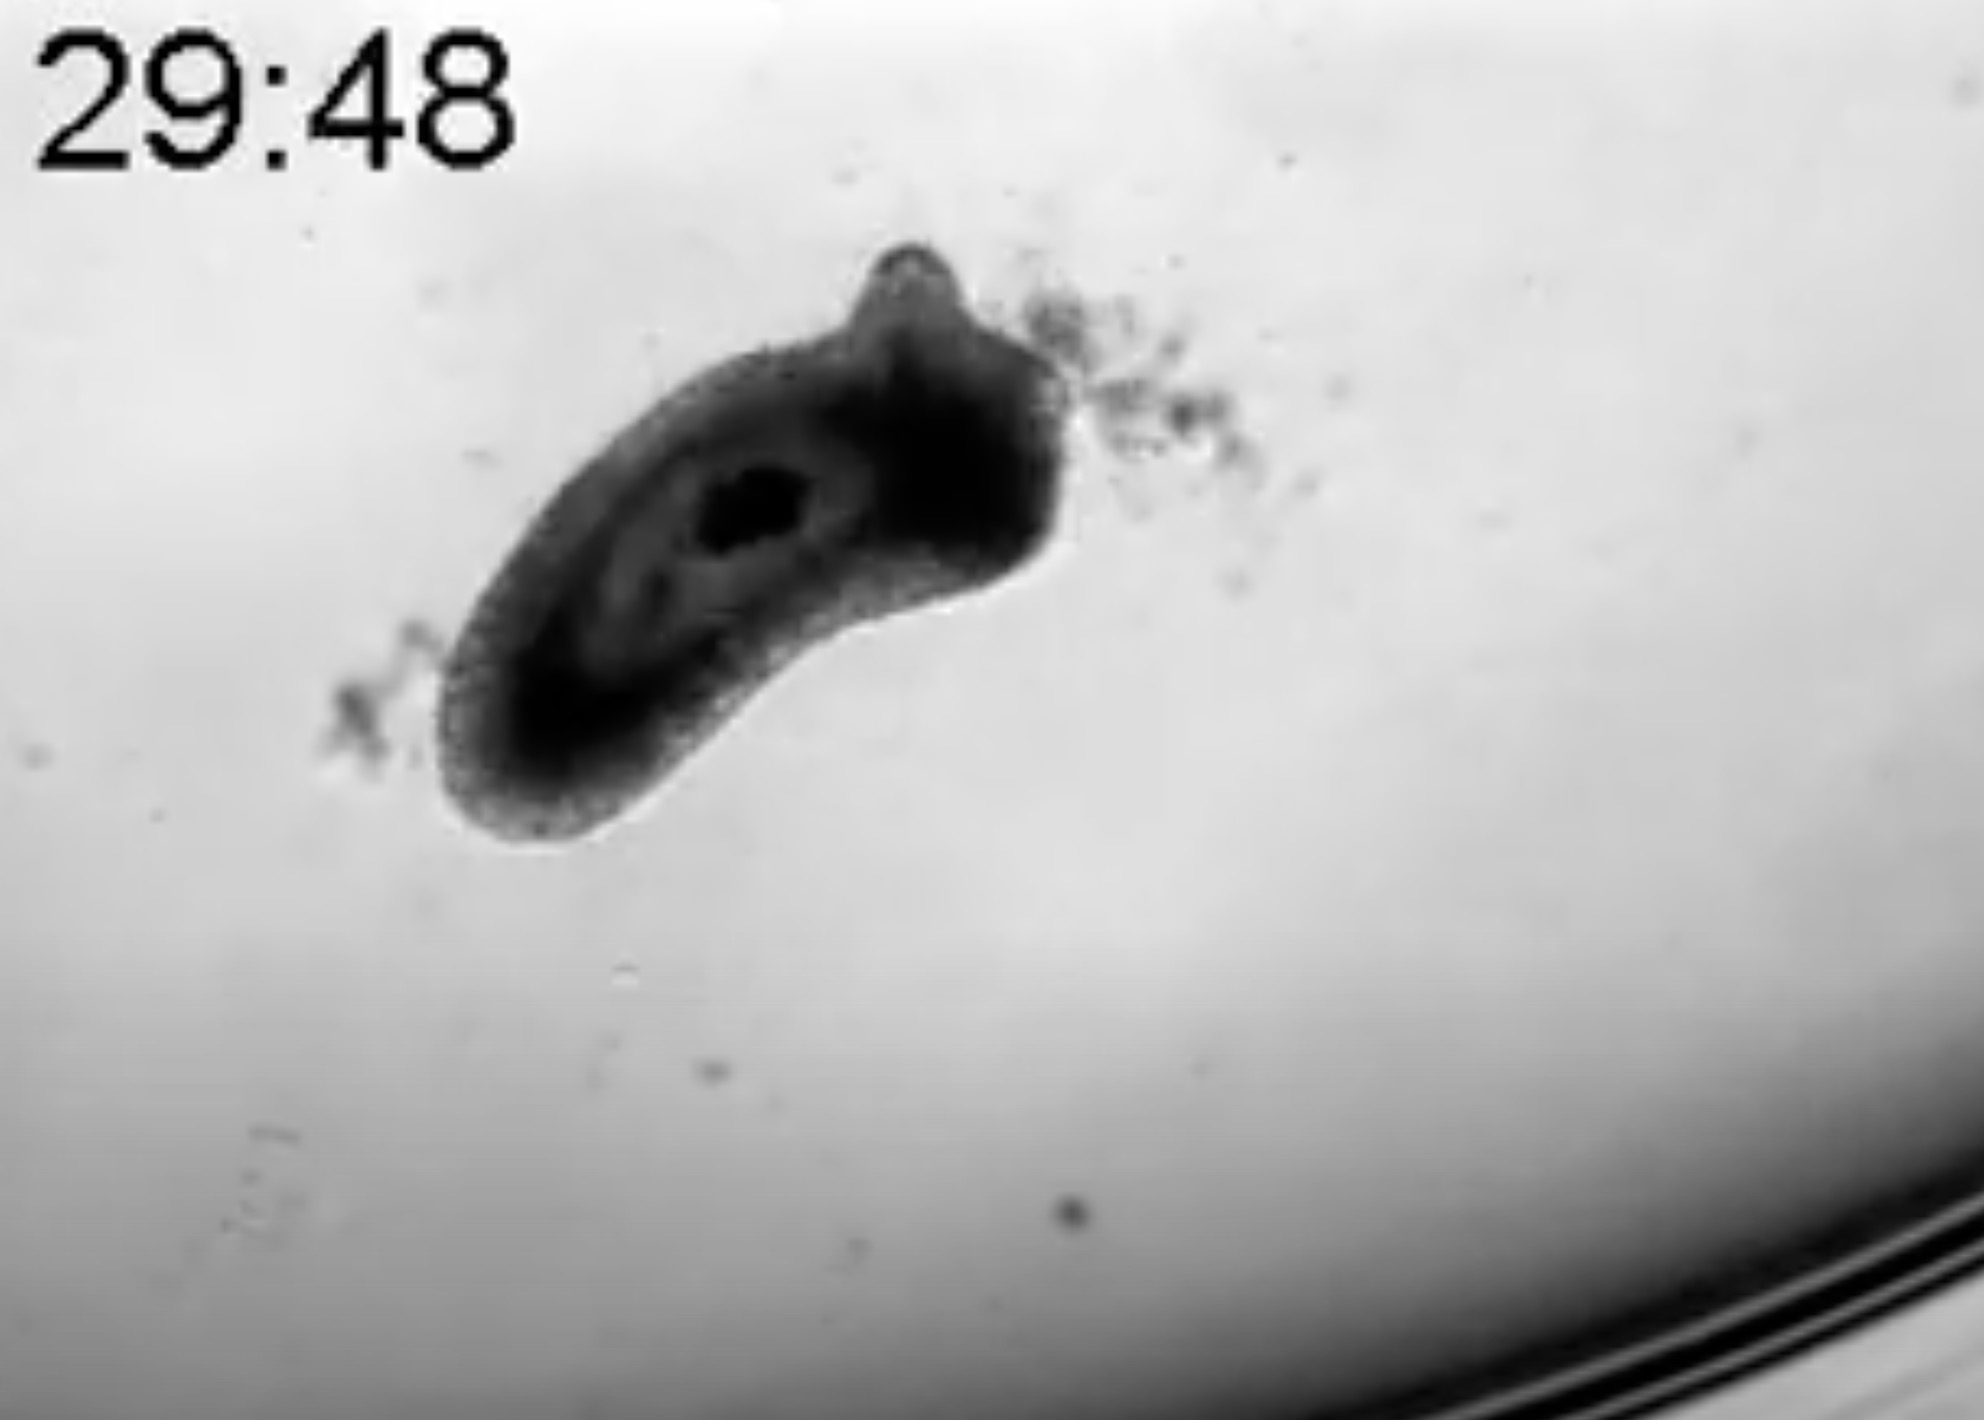
\includegraphics[width=0.19\textwidth]{figures/hydra_growth3}	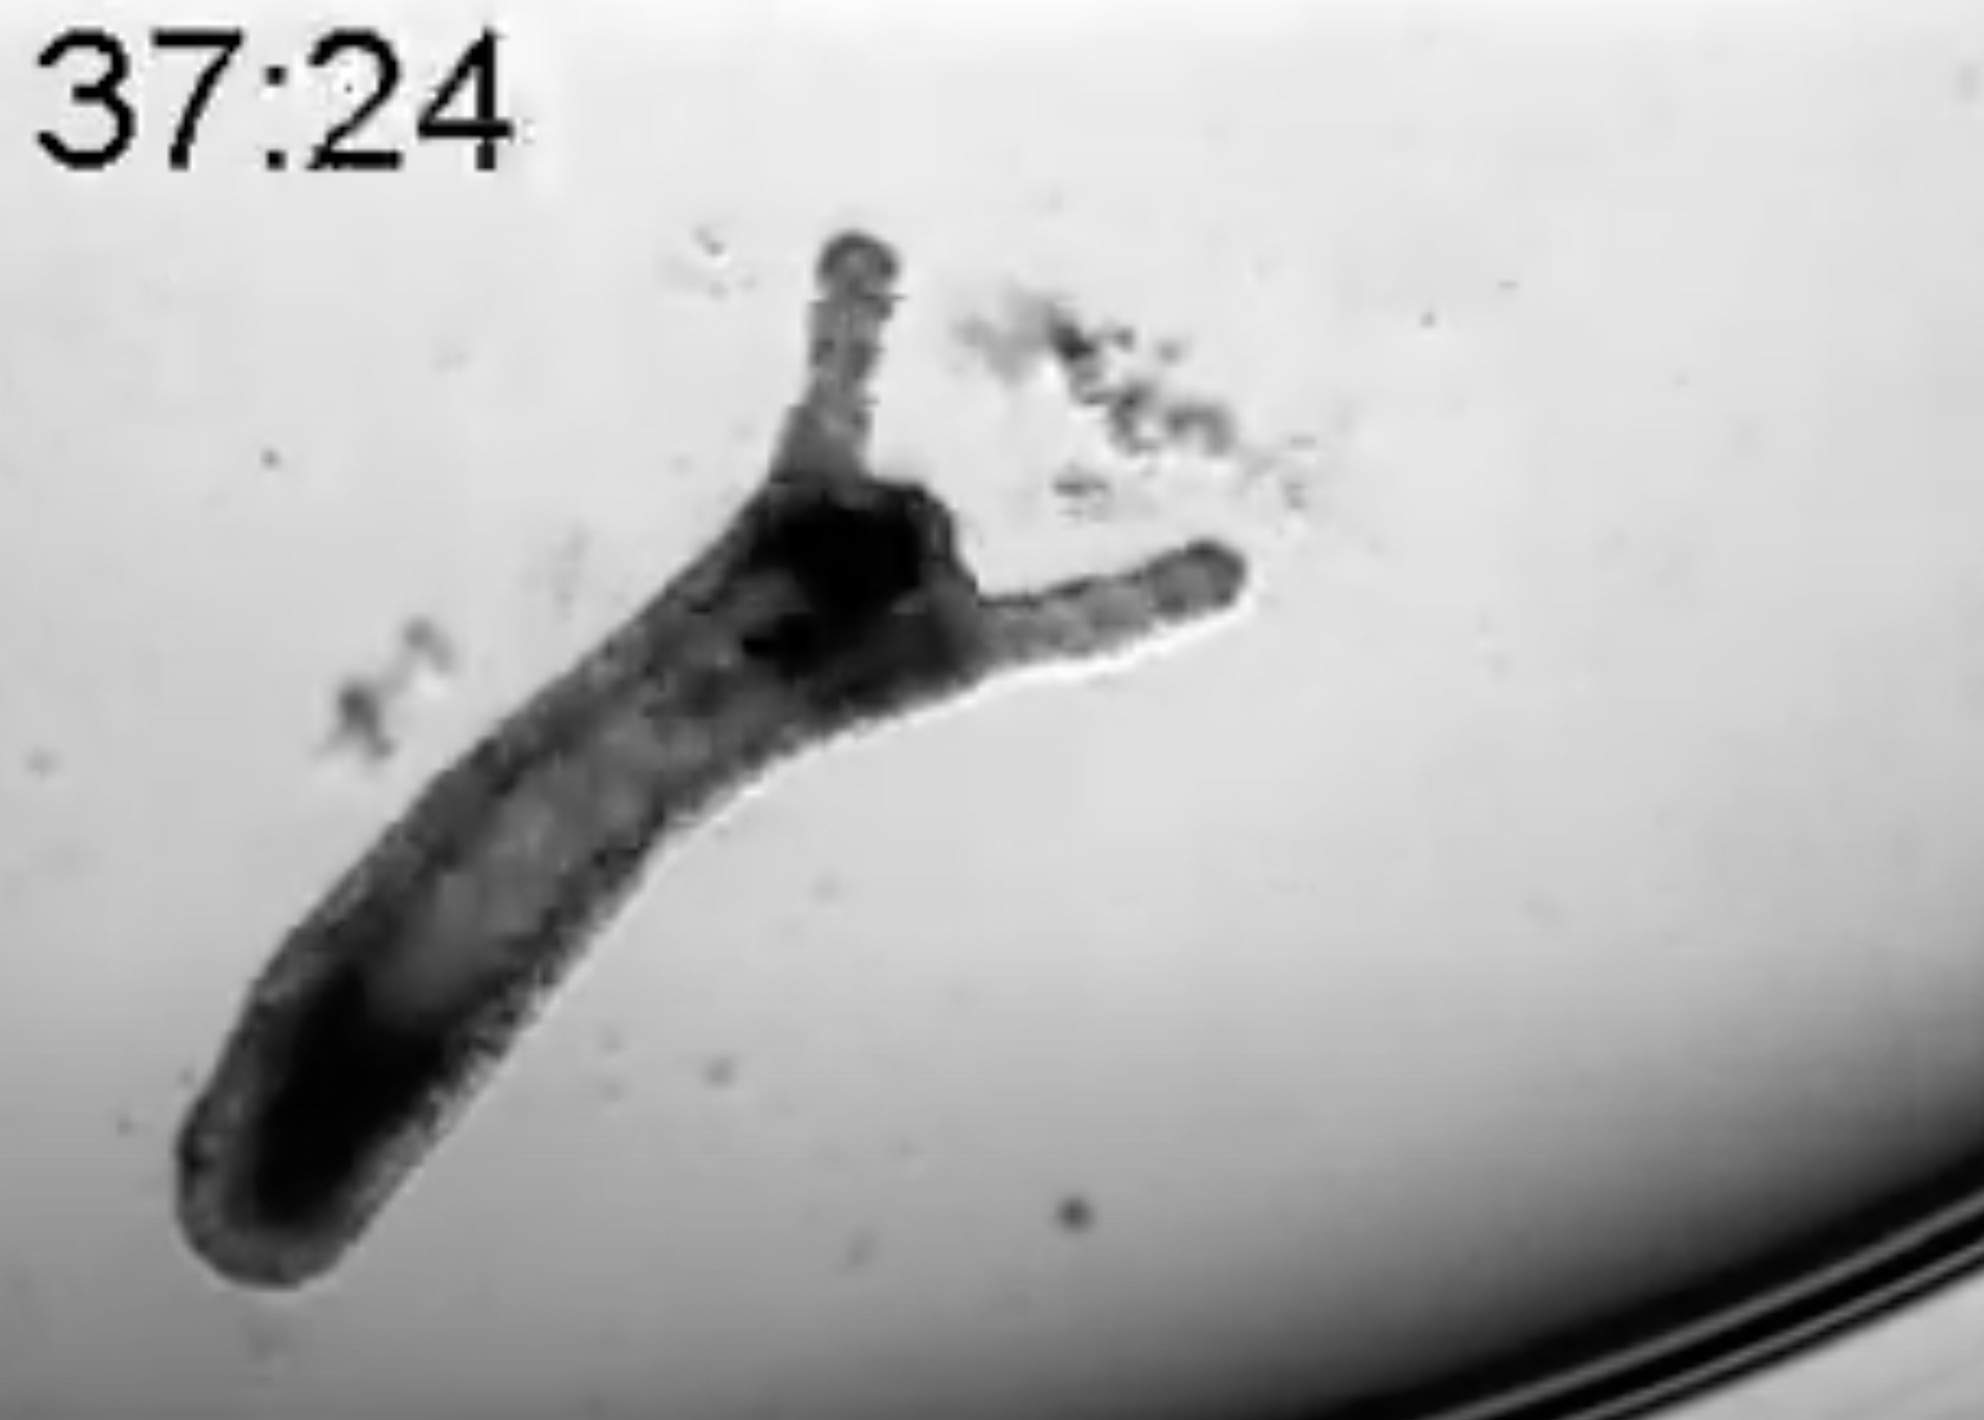
\includegraphics[width=0.19\textwidth]{figures/hydra_growth4}
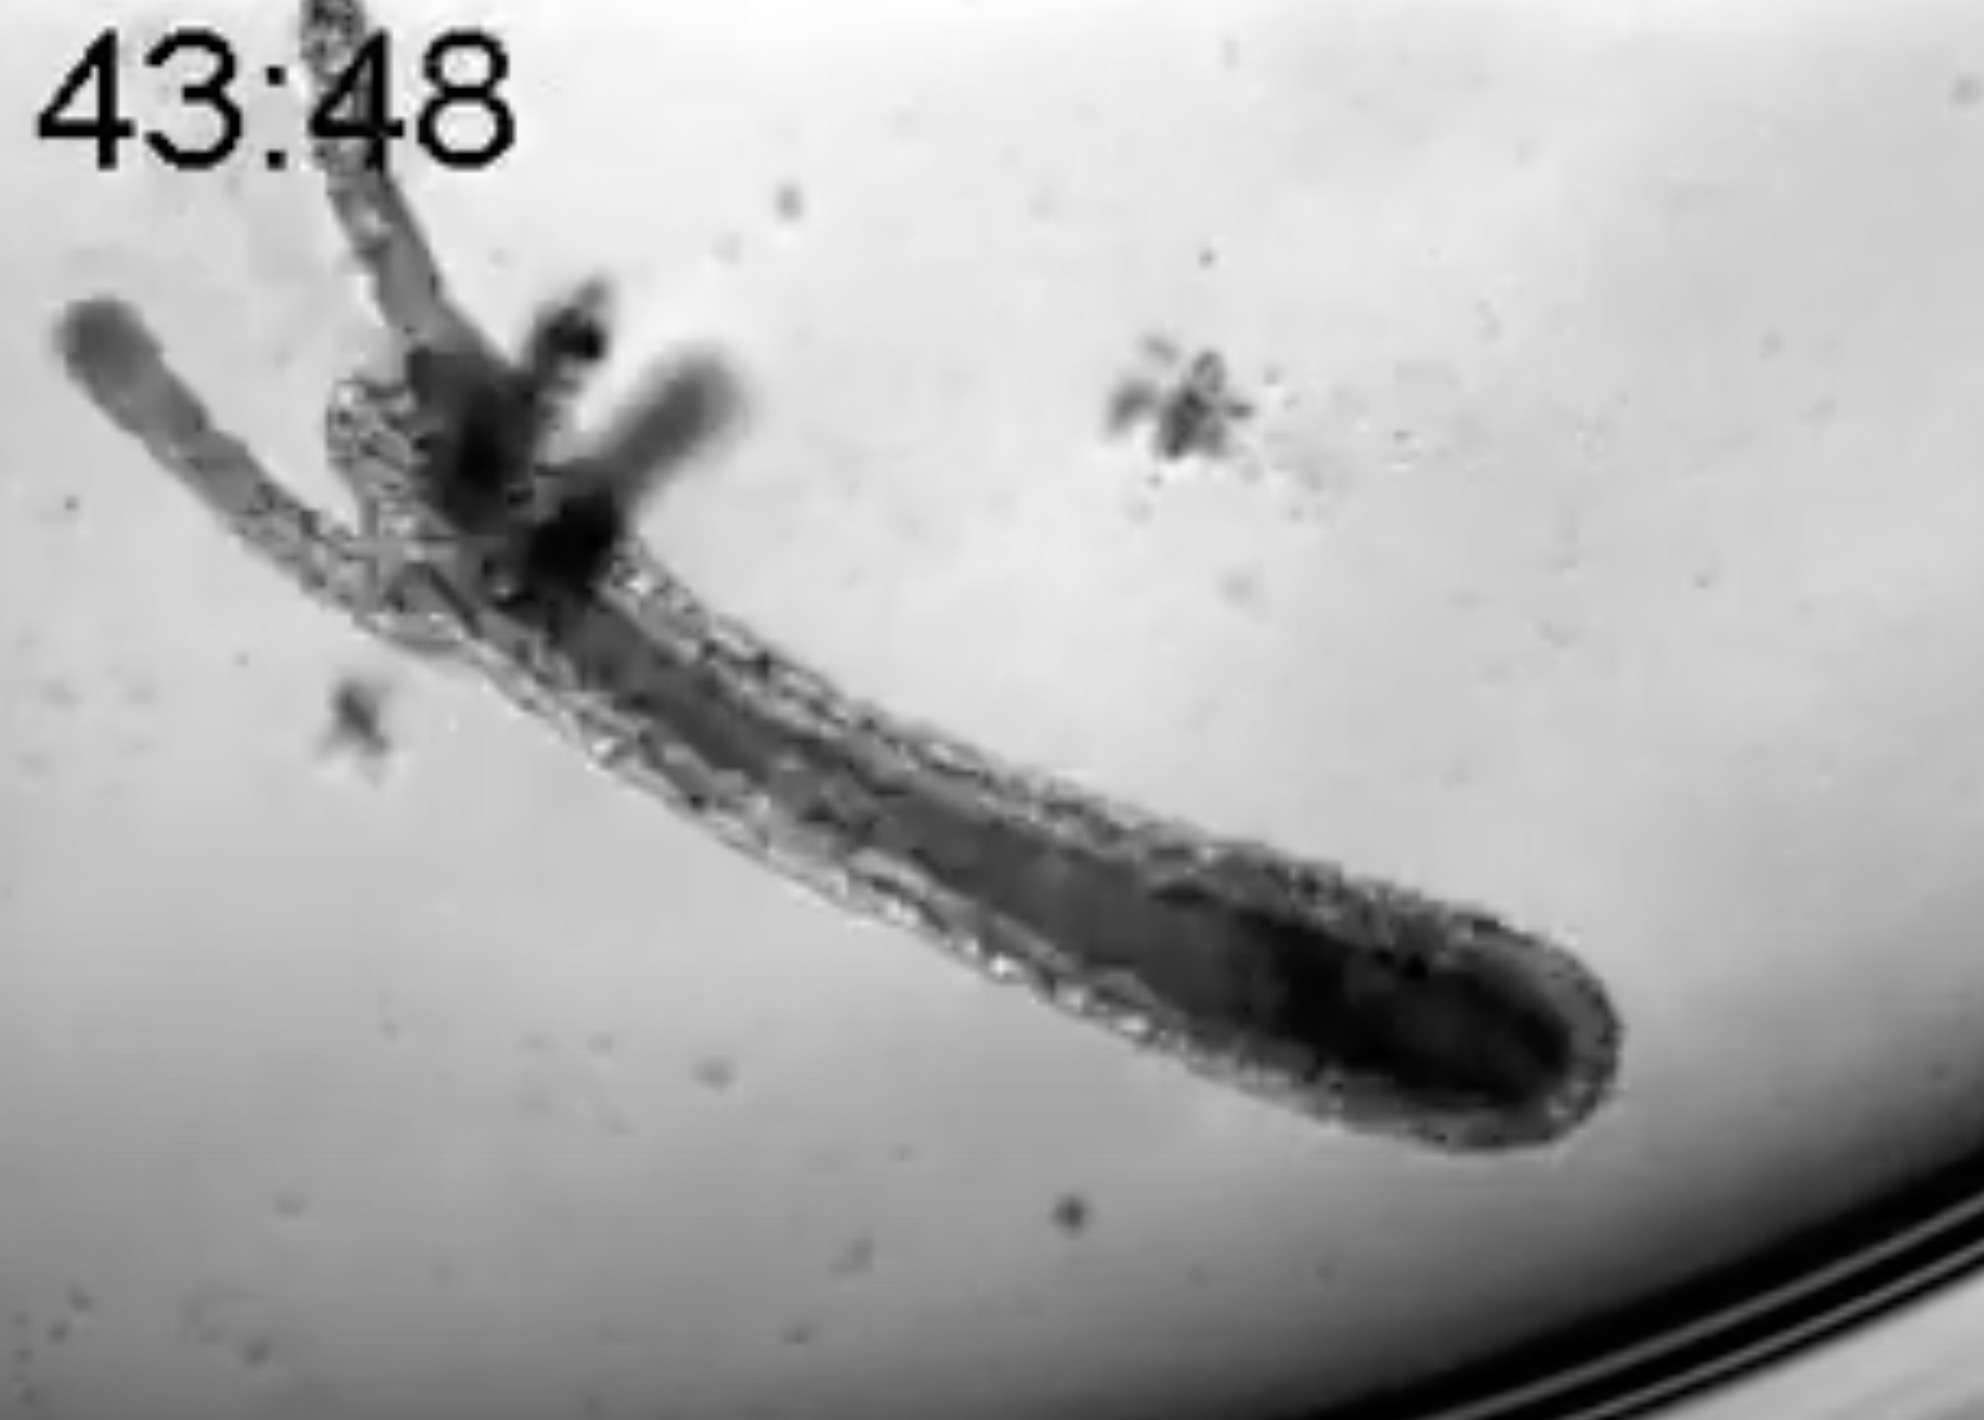
\includegraphics[width=0.19\textwidth]{figures/hydra_growth5}
\caption{Sequence of pictures taken under the microscope. It shows how Hydra is capable of regenerating its entire body from a small extracted sample of tissue coming from the body column (tissue diameter about 100 $\mu$m) of another Hydra. The timestamp on each picture is formatted as "hours:minutes", meaning the entire regeneration process takes place within two days only.}
\end{figure}

\subsection{The importance of Wnt signaling}

\section{Emergence of Patterns and Diffusion-Driven Instability}
How do patterns form? Pattern formation is the result of the collaboration of a large amount of biological processes ranging from the nanoscopic up to the microscopic scale. Together, they form motifs, which we define as the structural organization of cells in space and time, often leading to pretty shapes such as the fur coat in animals or that on the wings of a butterfly. In his pioneer paper  published in 1952 [\bref{ref}], Alan Turing proposes a chemical model for pattern formation involving two chemical species: one Activator ($u$), one Inhibitor ($v$) \incl{(Probably inspired from the Lotka-Volterra prey-predator model introduced in 1910 which was itself applied to mathematical biology for the first time in 1926)}. The concentration of each specie is described with 2-morphogens reaction-diffusion equations with appropriate boundary conditions, \textit{i.e.} equations of the form 


\begin{align}
	\del_t u &= d_1 \lap u + f(u, v) &\text{on} \ \R^{+} \times \Omega \notag \\[0.7em]
	\del_t v &= d_2 \lap v + g(u, v) & \text{on} \ \R^{+} \times \Omega \\[0.7em]
	\del_\nu u & = 0; \quad \del_\nu v = 0 & \text{on} \ \del\Omega \notag \\[0.7em]
	u(0, x) &= u_0(x) ; \quad v(0, x) = v_0(x) & u_0, v_0 \in X
\end{align}
\label{eq:TuringModel}


for a specific choice of $f$ and $g$ describing the chemical kinetics of the reaction. This choice is usually what determines the model type. To cite a few, we enumerate the Gray-Scott Model,  Gierer-Meinhardt, Fitzhugh-Nagumo , Bard-Lauder , Schnakenberg, Belousov-Zhabotinskii, the list goes on... [\bref{B. Perthame}]

